\documentclass[12pt,a4paper,conference]{IEEEtran}
\usepackage[utf8]{inputenc}
\usepackage[english]{babel}
\usepackage{amsmath}
\usepackage{amsfonts}
\usepackage{amssymb}
\usepackage{graphicx}
\usepackage{subcaption}

\usepackage{float}
\usepackage{fullpage}

\usepackage[hidelinks]{hyperref}

\usepackage{tikz}
\usepackage{fp} %floating point package

\usepackage{todonotes}
\usepackage{epstopdf}
\usepackage{graphicx}
\usepackage[T1]{fontenc}


\let\ig\includegraphics
\renewcommand{\includegraphics}[2][]{ \IfFileExists{#2}{ \ig[#1]{#2} }{ 
		\IfFileExists{#2.eps}{ \ig[#1]{#2} }{ 
		\IfFileExists{#2.png}{ \ig[#1]{#2} }{ 
		\IfFileExists{#2.jpg}{ \ig[#1]{#2} }{ 
		\IfFileExists{#2.jpeg}{ \ig[#1]{#2} }{ 
		\IfFileExists{#2.gif}{ \ig[#1]{#2} }{ 
		\IfFileExists{#2.ppm}{ \ig[#1]{#2} }{ 
		\missingfigure{  \protect\detokenize{#2} was not found.} 
}}}}}}}
}

\newcommand{\missingequation}[1]{\todo[inline, color = yellow]{Missing equation: #1}}


%%
%% End of file `mypackage.sty'.

\newcommand{\cutOutWidth}{0.45 \linewidth}
\newcommand{\histogramWidth}{0.8 \linewidth}
\newcommand{\fullImageWidth}{0.8 \linewidth}


\begin{document}
\raggedbottom

\title{Visual Servoing\\ \large{ROVI - Finalproject}}
\author{Nikolaj Iversen and Lukas Schwartz}
\date{18$^{th}$ December 2015}

\maketitle


\section{Feature Extraction}
%In order to make decisions based on images it is important to recognize objects.
In order to track an marker, it is important to detect these on an image when displayed.
%In order to test out different methods to find features, three different image markers were selected.
% Three image markers are given and the task is to find points that can represent the marker in the image.
In figure \ref{fig:markers} can the different markers to be tracked be seen.
In the simulation, the ideal marker is used but the markers will be tested on a set of real images where lighting, rotation and translation makes the markers harder to detect.
The detector should evaluate the image and return whether the marker was found, and either the center of the marker or several fixed points on the marker.
The detector should be invariant to translation, rotation and projection.
The goal is to use this to track a marker with a robot, keeping the marker in the center of the image and maintain the same distance.
Thus complete invariance to scaling is not a priority, but it should handle small changes in scaling.

\begin{figure}[h]
\centering
 \begin{subfigure}[b]{0.3\linewidth}
 \centering
 
\includegraphics[width=\linewidth]{graphics/Marker2a}
 \caption{Lines}
 \label{marker:cross}
 \end{subfigure}~
 \begin{subfigure}[b]{0.3\linewidth}
 \centering
 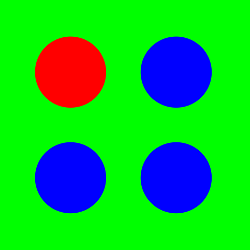
\includegraphics[width=\linewidth]{graphics/Marker1}
 \caption{Circles}
 \label{marker:circle}
 \end{subfigure}
 \begin{subfigure}[b]{0.3\linewidth}
 \centering
 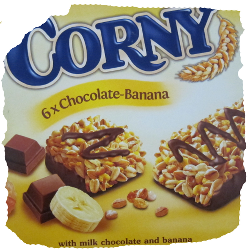
\includegraphics[width=\linewidth]{graphics/Marker3}
 \caption{Corny}
 \label{marker:corny}
 \end{subfigure}
 \caption{The different markers.}
 \label{fig:markers}
\end{figure}

% A full description of the choices and methods used to find the markers can be found in appendix \ref{app:full_vision_part}.
\subsection{The First Marker}\label{sec:full_marker1}
The first marker, seen in figure \ref{marker:cross}, contains black crossing lines on a white background.
These are two features which can be used to find the marker so both are tested.

Detection using lines was tested, but multiple lines occur in images.
With the used approach it was not possible to reliable detect the marker, so this approach was not considered further.
% so this was not deemed a good method.
The approach is described in appendix \ref{sec:using_lines}.

% \subsubsection{Using Contours}
% The second approach is to use the colors. 
Instead the colors were used.
The marker can be described as a big white rectangle, separated by black lines.
An initial separation of the possible markers is based on the size of the white elements found in the image.
%If the background contains small white blobs, the marker would be bigger.
%If the background is a big white wall, the size of the wall would be larger than the marker so that could be removed based on the size of the object.

The first problem is to find the white elements in an image.
Converting the image to grayscale and selecting threshold the high intensity is an option, but it does not handle shadows and bright areas well.
In figure \ref{fig:threshold_marker1} can the thresholded image be seen and the contours that are detected and within a set size constraint.
The red circle indicates where the marker is found.

\begin{figure}[H]
 \centering
 \begin{subfigure}{\exampleWidth}
 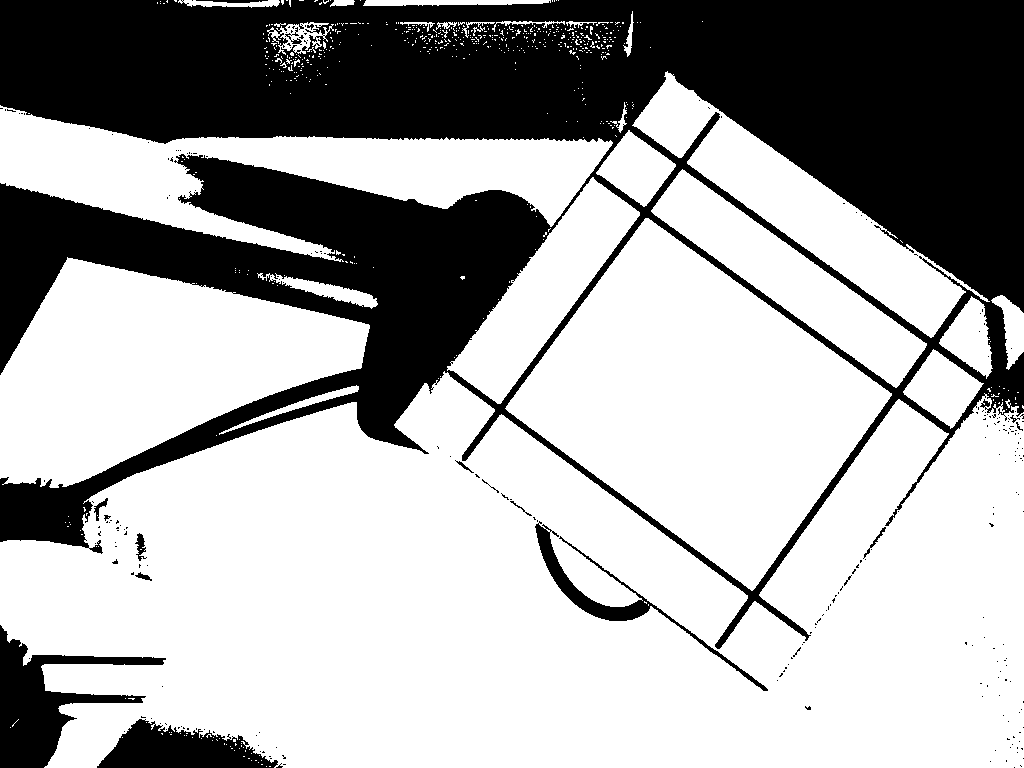
\includegraphics[width=\linewidth]{graphics/threshold_white}
 \caption{White in image.}
 \end{subfigure}
 \begin{subfigure}{\exampleWidth}
 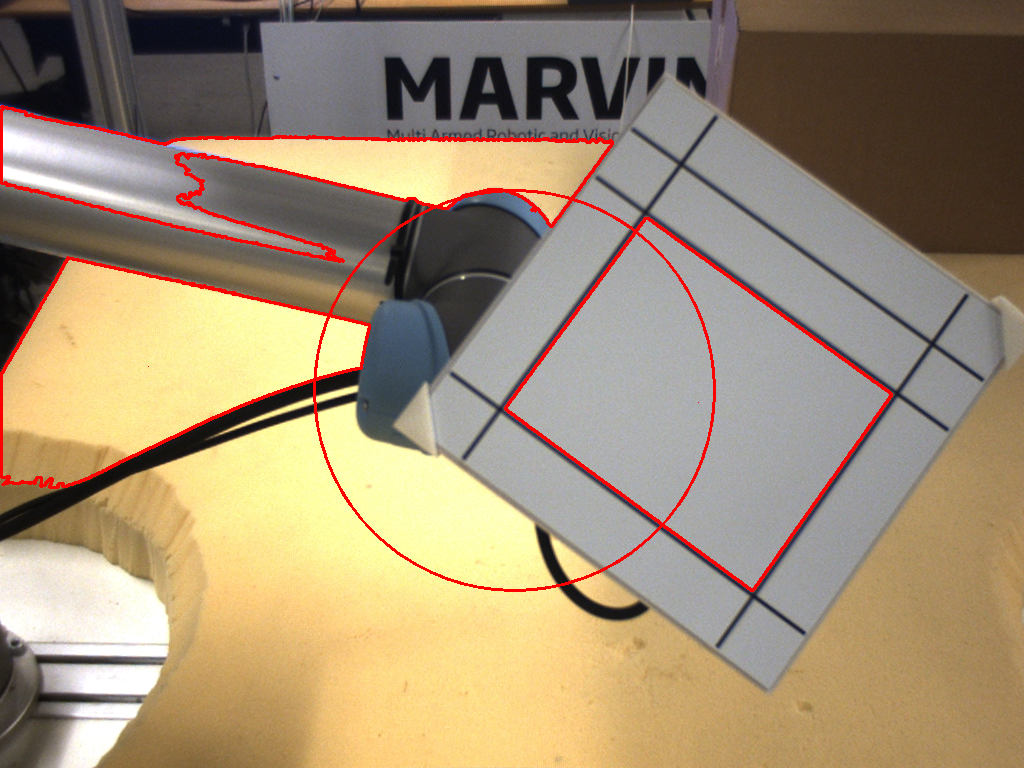
\includegraphics[width=\linewidth]{graphics/threshold_white_contours}
 \caption{Contours detected.}
 \end{subfigure}
 \caption{Detecting the white marker based on grayscale threshold.}
 \label{fig:threshold_marker1}
\end{figure}

%A better way to detect the white part is to split the image into the HSV colorspace.
To get a better result, the image was converted to HSV and perform the same approach as on the grayscale.
To threshold the image for only the white colors, the HSV values with 
%The value is the intensity of the image and selecting the high values gives the same effect as thresholding the grayscale image.
%To remove intense colored parts, the saturation must be set. 
%A low saturation would mean the image is not saturated with a color.
0-20\% saturation and 50-100\% intensity was chosen.
In figure \ref{fig:hsv_intensity} is the intensity shown in relation to the HSV values.

\begin{figure}[H]
\centering
 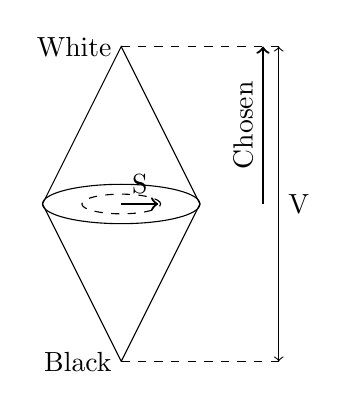
\begin{tikzpicture}
 \draw (0,0) -- (1,2) -- (0,4) -- (-1,2) -- (0,0);
 \draw (0,2) ellipse (1cm and 0.25cm);
 \node[left] at (0,4) {White};
 \node[left] at (0,0) {Black};
 \draw[dashed] (0,2) ellipse (0.5cm and 0.125cm);
 \draw[thick, ->] (0,2) -- ++(0.47,0) node[midway,above,name=s] {S};
 
 \draw[<->] (2,0) -- ++(0,4) node[midway, right] {V};
 \draw[thick, ->] (1.8,2) -- ++(0,2) node[midway, above,rotate=90] {Chosen};
 \draw[dashed] (0,0) -- (2,0) (0,4) -- (2,4);
 \end{tikzpicture}
 \caption[Saturation and intensity in relation to the HSV values.]{Saturation and intensity in relation to the HSV values. Saturation is not to scale in order to illustrate what is taken.}
 \label{fig:hsv_intensity}
\end{figure}


In figure \ref{fig:hsv_marker1} are the white parts and the contours shown for the same area constraints as in figure \ref{fig:threshold_marker1}.
%The HSV values are more robust to changes in the environment and is thus better suited for this assignment.
The HSV values are more reliable at finding true white and is thus better suited for this approach.

\begin{figure}[H]
 \centering
 \begin{subfigure}{\exampleWidth}
 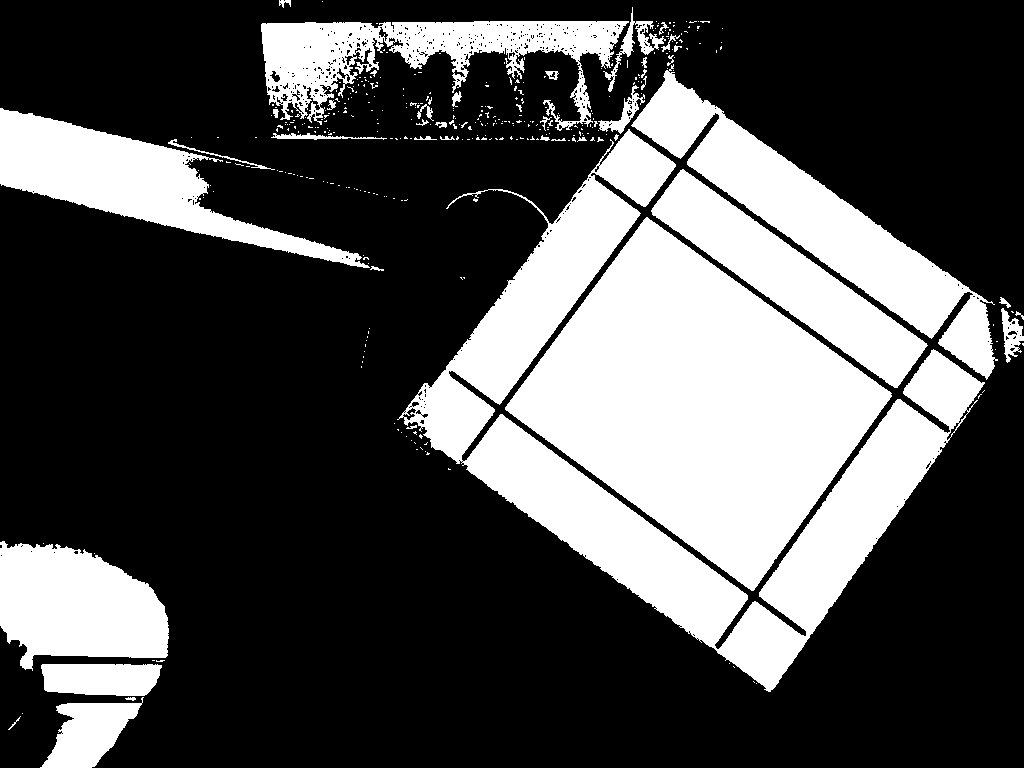
\includegraphics[width=\linewidth]{graphics/hsv_white}
 \caption{White in image.}
 \end{subfigure}
 \begin{subfigure}{\exampleWidth}
 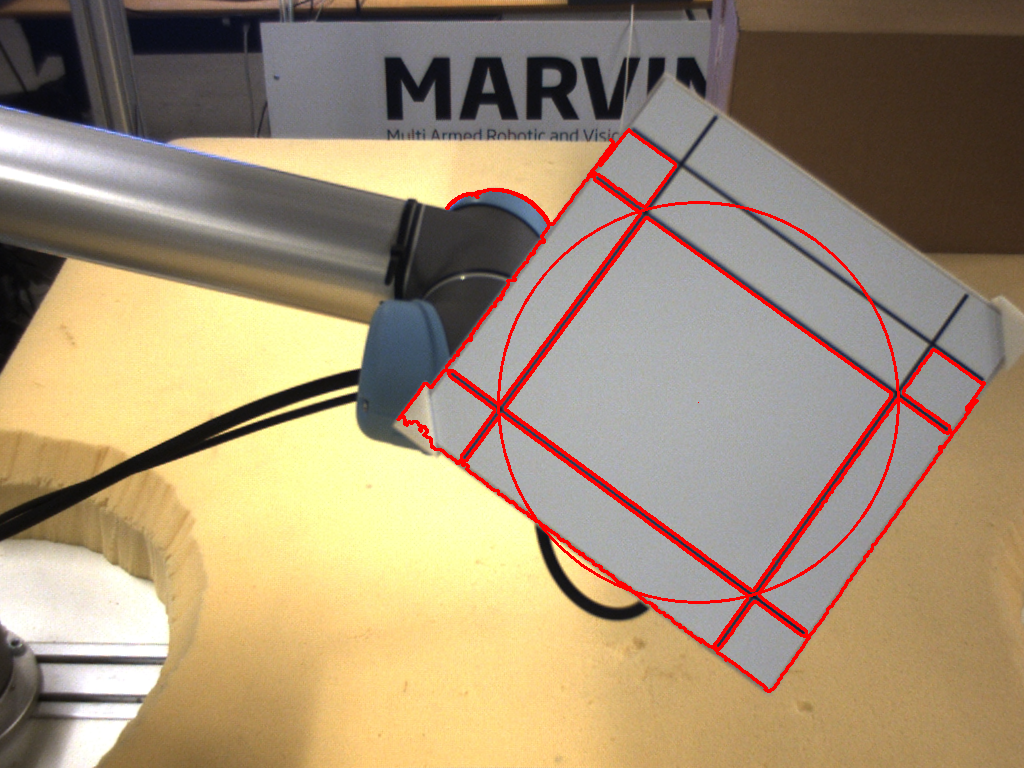
\includegraphics[width=\linewidth]{graphics/hsv_white_contours}
 \caption{Contours detected.}
 \end{subfigure}
 \caption{Detecting the white marker based on HSV threshold.}
 \label{fig:hsv_marker1}
\end{figure}

When the white parts of an image has been detected, the blobs can be found.
%By calculating the areas within the contours, the parts within the size of the marker can be found.
Once found, the center of the marker is found by taking the most compact contour that is closest to the center of the image.
As the robot will be following the position of the marker, this is a good estimate, but it also proved to be good in the images used in the test set as the distracting blobs were not placed in the center, behind the marker.
Using this approach the marker can be found on all the images in the easy and hard set.
To select the appropriate blob as the marker, the both the compactness and the distance to from the center are normalised to a value between zero and one, where one is close to the center and very compact.
The two properties are then scaled and the blob with the highest value is chosen, if it is greater than a minimum threshold.
%\nikolaj{Should I test how many times the marker is found in images where the marker is not there?
%I think it might just always detect the marvin sign or something similar.}
The center of mass is then returned as the position of the marker to be used for the tracking.

\subsection{The Second Marker}
The second marker, seen in figure \ref{marker:circle}, contains three blue circles and one red circle in a green square.
First the image is split into a red, green and blue channel using HSV.
When using HSV to select for colors, hue is the dominating factor.
%The hue is selected by giving an interval in degrees from the circle.
The hue is selected as shown in figure \ref{fig:hsv_color_segmentation}.
The saturation is chosen so it selects high values as saturated red, green and blue is desired.
The intensity is not important as the ideal marker gives full intensity of the colors and the real images will give a lower intensity.

\begin{figure}[h]
\centering
\def\scalingFactor{0.4}
\begin{tikzpicture}[scale=\scalingFactor, every node/.style={scale=\scalingFactor}]
 \node[name=whole] at (-0.12,-0.05) {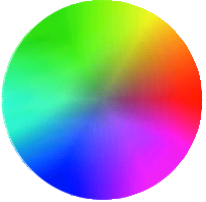
\includegraphics[scale=1]{graphics/hue} };
\end{tikzpicture}
%
\begin{tikzpicture}[scale=\scalingFactor, every node/.style={scale=\scalingFactor}]
\node at (0,-2.2) {};
\node at (0, 2.2) {};
\def\startAngle{140}
\def\stopAngle{50}
  \draw[rotate=5,fill=gray,line width=1pt] (\startAngle:1cm) arc(\startAngle:\stopAngle:1cm) -- (\stopAngle:1.125cm) -- (0.9,0.4) -- (\stopAngle:.625cm) -- (\stopAngle:.75cm) arc (\stopAngle:\startAngle:.75cm)--cycle;
\end{tikzpicture}
%
\begin{tikzpicture}[scale=\scalingFactor, every node/.style={scale=\scalingFactor}]
 \node at (-0.12,-0.05) {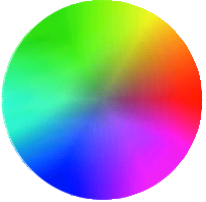
\includegraphics[scale=1]{graphics/hue} };
 \node[name=hsv, draw, thick , circle, minimum width =5.3cm] at (0,0) {};
% % % % RED % % % %
\def\MaxSat{2.8cm}
\def\MinHueR{0} 
\def\MaxHueR{30}
\def\MinSatR{1.6cm} % 0 - 1 => 0 - 2.65
 \draw (hsv.\MinHueR) -- (hsv.center) -- (hsv.\MaxHueR);
 \draw[very thick]   ([shift=(\MinHueR:\MinSatR)] hsv.center) arc(\MinHueR:\MaxHueR:\MinSatR);
% % % % GREEN % % % %
\def\MinHueG{70} 
\def\MaxHueG{145}
\def\MinSatG{1.6cm} % 0 - 1 => 0 - 2.65
 \draw (hsv.\MinHueG) -- (hsv.center) -- (hsv.\MaxHueG);
 \draw[very thick]   ([shift=(\MinHueG:\MinSatG)] hsv.center) arc(\MinHueG:\MaxHueG:\MinSatG);
% % % % BLUE % % % %
\def\MinHueB{210} 
\def\MaxHueB{270}
\def\MinSatB{1.6cm} % 0 - 1 => 0 - 2.65
 \draw (hsv.\MinHueB) -- (hsv.center) -- (hsv.\MaxHueB);
 \draw[very thick]   ([shift=(\MinHueB:\MinSatB)] hsv.center) arc(\MinHueB:\MaxHueB:\MinSatB);

 \fill[color=white]  (hsv.center) -- (0:\MinSatR) arc(0:360:\MinSatR);
 
 \fill[color=white]  (hsv.center) -- (\MaxHueR:\MaxSat) arc(\MaxHueR:\MinHueG:\MaxSat);
 \fill[color=white]  (hsv.center) -- (\MaxHueG:\MaxSat) arc(\MaxHueG:\MinHueB:\MaxSat);
 \fill[color=white]  (hsv.center) -- (\MaxHueB:\MaxSat) arc(\MaxHueB:360:\MaxSat);
\end{tikzpicture}
\caption{Hue and Saturation thresholds applied to HSV to segment colors.}
\label{fig:hsv_color_segmentation}
\end{figure}

The circles are then found by using a Hough transform for circles on the green channel.
The green channel will create a void, and thus edges, where the red and blue circles are found so this is less expensive than finding circles on two colors.
During evaluation of this method, it was found that this method sometimes missed a red or a blue circle.
This could be saved by doing an extra Hough transform on the corresponding channel and find the circle there.

In order to deal with projection, the Hough transform must allow more edges to be viewed as circles.
This means that more points will be found.
In order to remove the wrong points, the surrounding points are analyzed, and if found not to be green, the circle is removed.

The detector was tested to find 4 correct points in the marker in 30/30 images in the easy set and in 50/52 images in the hard set.

In figure \ref{fig:circle_detection} is a normal case from the easy and a worst case example from the hard set shown.
As the robot follows the point, it is not expected to be this bad at any situation so the detector is deemed successful.

\begin{figure}[h]
 \centering
 \begin{subfigure}{0.49\linewidth}
 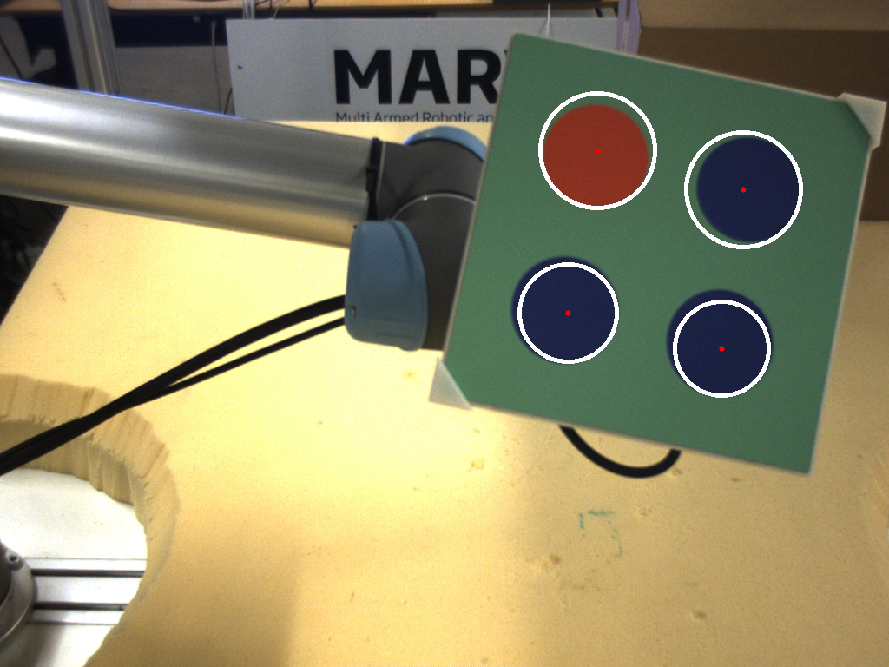
\includegraphics[width=\linewidth]{graphics/best_case_hough_circle}
 \caption{Normal case.}
 \end{subfigure}
 \begin{subfigure}{0.49\linewidth}
 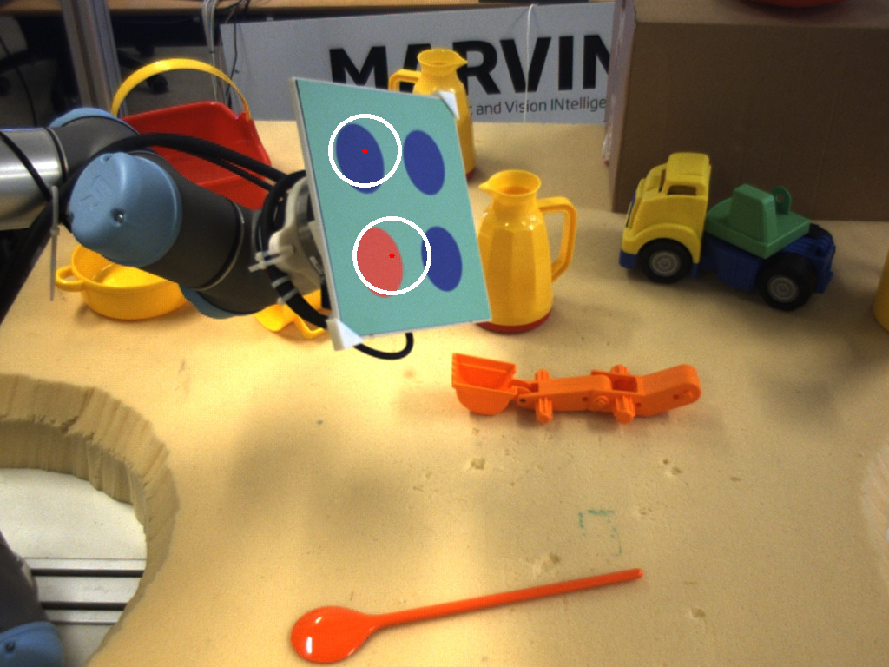
\includegraphics[width=\linewidth]{graphics/worst_case_hough_circle}
 \caption{Worst case.}
 \end{subfigure}
 \caption{Detecting circles with and without projection.}
 \label{fig:circle_detection}
\end{figure}



\subsection{The Third Marker}
The third marker, seen in figure \ref{marker:corny}, contains an image of packaging from a granola bar.
Here the colors are not distinct enough to use as the source and there is no good definable shapes in the image worth searching for.
In those situations can the Scale Invariant Feature Transform (SIFT) be used.
SIFT points in an image which then can be matched to the marker.
\nikolaj{I should probably describe some more about SIFT here, I will do research on it later}

Once the features are extracted, they can be inserted into a search tree using FLANN.
FLANN makes a balanced binary search tree so the features in the scene and the features in the marker can be matched.
Then the matches are compared using RANSAC and the corners of the marker is projected onto the image. 

To test if the marker is successfully detected, lines between the corners have been drawn onto the image.
In figure \ref{fig:sift_detection} can it be seen that the marker is successfully detected.

\begin{figure}[h]
 \centering
 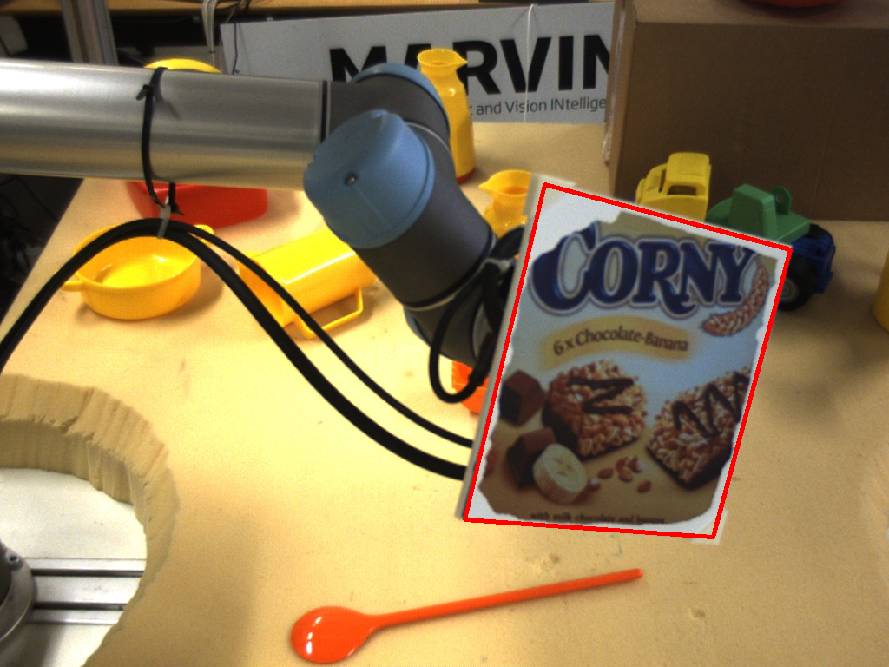
\includegraphics[width=0.5\linewidth]{graphics/sift_detection}
 \caption{SIFT detection on an image.}
 \label{fig:sift_detection}
\end{figure}

Testing the performance of SIFT shows that it successfully detected 30/30 images on the easy set and 52/52 images on the hard set.
To measure the performance of SIFT, the timing was measured. 
The timing is shown in figure \ref{fig:time_sift_unoptimized}. 
The timing of calculating SIFT takes $665$ ms on average to detect the marker.
This can be a problem if a robot should react on a moving object.
The timing is split into three problems, the time it takes to find the keypoints, the descriptors and the homography.
The homography can be faster by reducing the number of matches.
This could be done by removing matches that deviate from the minimum distance between two features.
\nikolaj{Find if this is pixel distance between them or something else}
Running with this optimization, the total time goes down to a $630$ ms on average.

\begin{figure}[h]
 \centering
 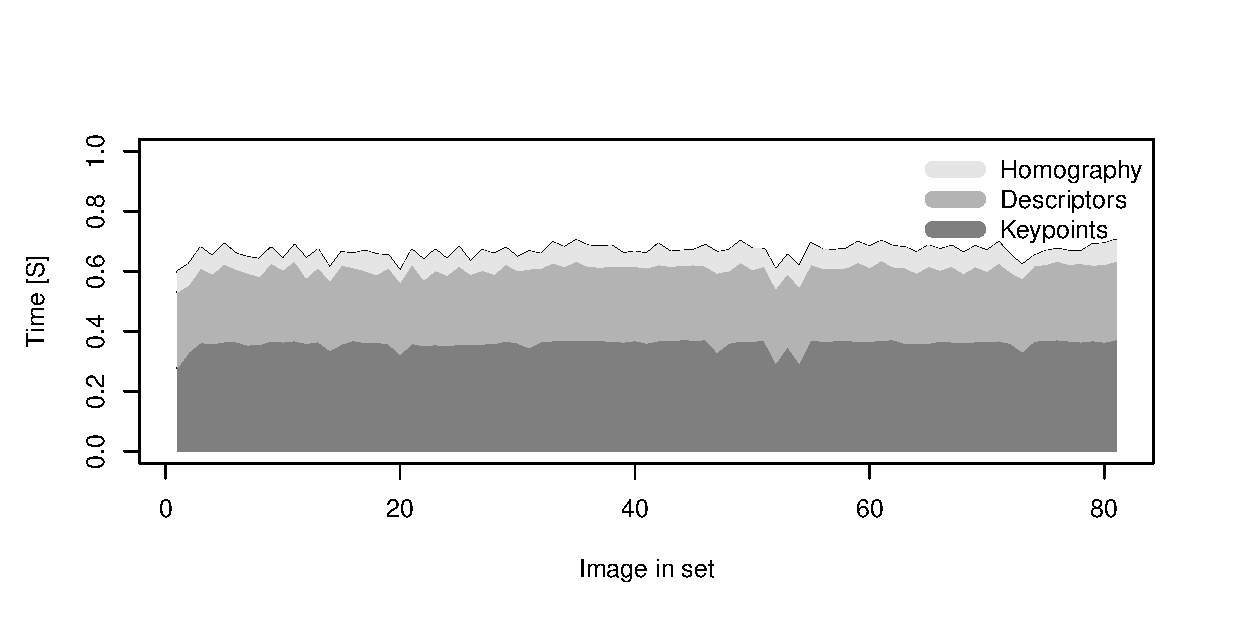
\includegraphics[width=\linewidth]{graphics/marker3_timing_unoptimized}
 \caption{Timing for finding the marker with SIFT.}
 \label{fig:time_sift_unoptimized}
\end{figure}

In figure \ref{fig:time_sift_unoptimized} it can be seen that calculating the SIFT features is what is taking the majority of the time.
A way to reduce this is to reduce the image by cropping.
Since the scenario is that the robot will track the marker, the marker can be expected to be in the same position all the time.
Since the distance to the object does not change drastically, the marker will keep the same size in relation to the image.
By using the last known position of the marker and cropping it, the time to find the SIFT features can be reduced.
If the marker is not found, as it would be the case if the marker has moved too far out of frame, the entire picture should be used for the next analysis.
This would also be the case for the first image, as the position starts as unknown.

In figure \ref{fig:time_sift_crop} is the timing shown for the finding the marker, using the cropping optimization.
The timing now has outliers as it takes more time to process the larger image.
The median is then found to in order to estimate the time it takes to find the marker with the optimized solution.
The median is measured to be $272$ ms.
The large image is analyzed two times, one for the first image and one for image 28 as the transition from 26 to 27 is not continuous.
The transition from the easy image set to the hard image set is continuous enough so the detector finds the marker.

\begin{figure}[h]
 \centering
 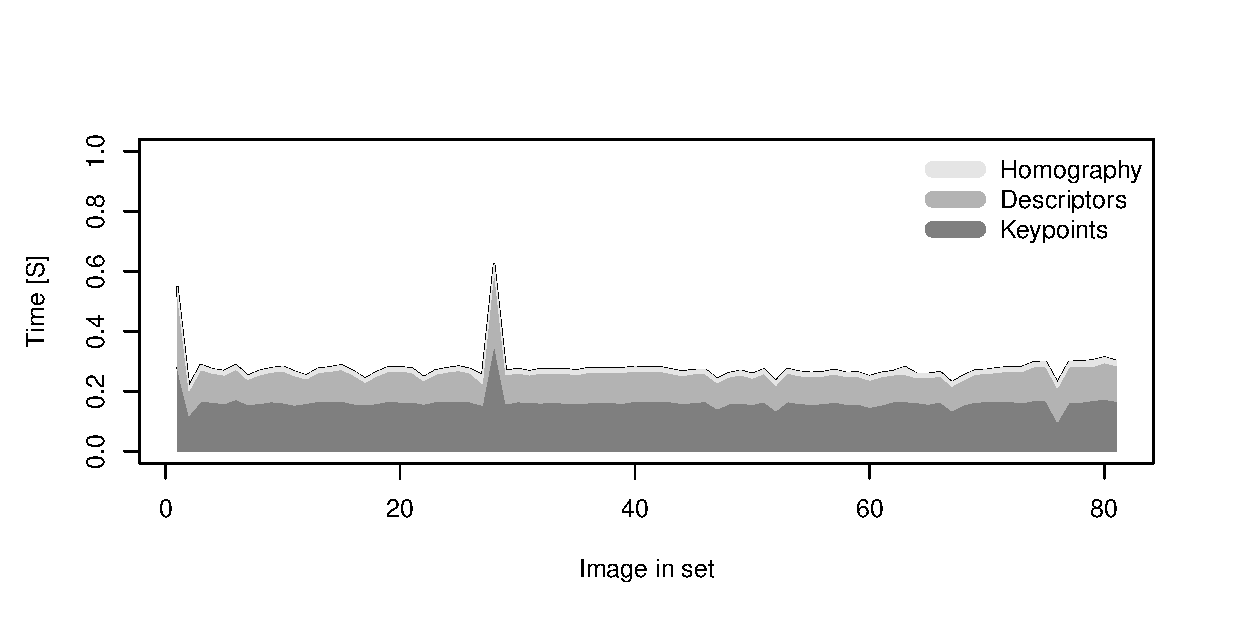
\includegraphics[width=\linewidth]{graphics/marker3_timing_crop}
 \caption{Timing for finding the marker with SIFT optimized for servoing.}
 \label{fig:time_sift_crop}
\end{figure}


\subsection{Conclusion}
An algorithm was found to locate the three markers in an image.
A set of points was then chosen to represent the position of the marker to be used by the tracking algorithms.

The line marker was found using HSV color segmentation for white after which contours were found.
The blobs were then given a grade depending on their compactness and distance to center.
Depending on their grade, the marker was then detected or not.
This was very optimistic and found a fast solution, but also found solutions in images where the marker is not present.

For the circle marker a HSV color segmentation was applied to find a green, blue and red image.
Hough circles was then applied to find the circles surrounded by green.
If the marker was not found in the green image, the circles were also searched for in the blue and red image.

The corny marker was found using SIFT.
The processing time was furthermore improved using cropping on the image depending on the locality of the marker.


%The markers were found to detect the presence of the individual markers.

%Marker one is detected as the center of the white parts of the image.
%Marker two is detected as the center of the circles of the image.
%Marker three is detected as the corners of the marker.

\begin{figure}
\begin{tikzpicture}
 \newcommand{\angleA}{10}
 \newcommand{\radiuA}{1}
 \newcommand{\radiuB}{1}
 
 \FPeval{\angleB}{\angleA + 90}
 
 \node[name=image] at (0,0) {};
 
 \node[scale=0.3,fill=black, minimum width=15cm, rotate={90 + \angleA}, name=lineA] at ([shift=(\angleA:\radiuA cm)] image.center) {};
 \node[name=midA] at ($(wall.180)!(image.center)!(wall.0)$) {};
 \node[above] at (lineA.0) {line a};

 \node[scale=0.3,fill=black, minimum width=15cm, rotate={90 + \angleB}, name=lineB] at ([shift=(\angleB:\radiuB cm)] image.center) {};
 \node[name=midB] at ($(wall.180)!(image.center)!(wall.0)$) {};
 \node[above] at (lineB.0) {line b};
 
 \FPeval{\rad}{\FPpi/180} %couldn't find the function
 \FPeval{\posX}{round(cos(\angleA * \rad)*\radiuA + cos(\angleB * \rad)*\radiuB,3)}
 \FPeval{\posY}{round(sin(\angleA * \rad)*\radiuA + sin(\angleB * \rad)*\radiuB,3)}
 
 \node[draw, circle]  at (\posX,\posY) {};
\end{tikzpicture}
\end{figure}

\section{Point Tracking}
When doing Visual servoing, a point is followed by the robot.
In this report the tracking is done using a single camera on a simulated robot in RobWorkStudio.
First the case where the robot tracks a single point is considered, followed by the tracking of multiple points.
\subsection{Tracking a Single Point}
In order to track a single point, then the equations \ref{eq:tsp_visServoing1} and \ref{eq:tsp_visServoing2} (cite Henriks notes) were implemented.

\begin{eqnarray}
(Z_{image} \cdot Z_{image}^T) y = [du, dv]^T \label{eq:tsp_visServoing1} \\
dq = Z_{image}^T \cdot y \label{eq:tsp_visServoing2}
\end{eqnarray}

Furthermore a time scaling was implemented such that the robot would not move faster than its constraints.
The goal configuration for each frame is furthermore stored such that when a marker is not found in one frame, then the most recent found position is the one the robot moves to.

In order to test the implementation of the algorithm, the marker movement of the three files are stepwise used to update the markers position.
The $dq$ for every step is then computed and used to update the robot.

To find the simulated $(u,v)$ of the marker in the frame of the camera, then the transformation from the camera to the marker ($T_{world}^{camera}$) is found using equation \ref{eq:tsp_TcameraMarker}.

\begin{equation}
T_{world}^{marker} = T_{world}^{camera} \cdot T_{camera}^{marker} \label{eq:tsp_TcameraMarker}
\end{equation}

From $T_{camera}^{marker}$ the positional part is then extracted and used with equation \ref{eq:tsp_u} and \ref{eq:tsp_v} to find $(u,v)$ using the pinhole model.
Where $f$ is the focal length in pixel.

\begin{eqnarray}
u = \frac{f \cdot x}{z} \label{eq:tsp_u} \\
v = \frac{f \cdot y}{z} \label{eq:tsp_v}
\end{eqnarray}


\subsubsection{Testing the Point Tracking}

The system was tested on the three marker movements provided and the configuration of the robot is plotted in figure \ref{fig:robotconfig_ideal}.
The tool pose was likewise plotted in figure \ref{fig:toolpose_ideal}.

\begin{figure}[H]
\centering
\includegraphics[width= 0.9 \linewidth]{graphics/robotconfig_ideal}
\caption{Robot configuration when calculating the ideal $(u,v)$ for the marker placement in the image.}
\label{fig:robotconfig_ideal}
\end{figure}

\begin{figure}[H]
\centering
\includegraphics[width= 0.9 \linewidth]{graphics/toolpose_ideal}
\caption{Tool pose when calculating the ideal $(u,v)$ for the marker placement in the image.}
\label{fig:toolpose_ideal}
\end{figure}


Since these numbers should be the closest to ground truth achievable, then these will also be used in comparisons in section \ref{sec:combinedSystem} when the whole system is brought together in the simulation.

It was found that in none of the cases was the velocity constraint violated for all of the datasets down to a $\Delta t$ of 0.05 seconds in between each frame.



\subsection{Tracking Multiple Points}


\subsection{Conclusion}

\section{Combined Feature Extraction and Tracking}
To see how the system performed when the modules have been combined, the three vision algorithms were all implemented into the plugin.
A set of different backgrounds was used to see the robustness of the detectors.
In appendix \ref{app:scenes} can the different backgrounds be seen.

The time it takes to find the marker is measured and subtracted from the time the robot has to move to the point.
This means that the robot will meet the velocity constraints and loose the target if the marker moves too fast.
\subsection{Tracking the Points}
The velocity constraint was furthermore limited to only compute the robot movement from the time left over by the vision algorithm.
It is hence assumed that when the time limit $\Delta t$ is exceeded by the vision algorithm, the result of the process is not used.
The time by which $\Delta t$ is reduced, is calculated on runtime and hence dependent on the time it takes to process the specific image.

The slow data set contains 500 points, the medium, 160, and the fast data set contains 50 points.
In order to minimize the effect of outliers, the number of trials is increased on the data sets which have less data points.

The time to find the marker is measured and the mean processing time is shown in table \ref{tb:mean_processing_time}.
The different backgrounds was tested separately to see if it has any impact.
It can be seen that the Corny detector takes more time on backgrounds such as carpet and mosaik window, as they contain a lot of edges and thus a lot of SIFT features.

\begin{table}[H]
\center
\begin{tabular}{|l|*{3}{D{.}{.}{2}|}}
\hline
Background       & Line  & Circles & Corny  \\ \hline
None             & 30.02 & 39.87   & 234.14 \\ \hline
Many Butterflies & 31.38 & 48.13   & 280.96 \\ \hline
Color Spots      & 32.18 & 42.33   & 262.47 \\ \hline
One Butterfly    & 32.17 & 46.75   & 306.68 \\ \hline
Metal            & 33.31 & 42.02   & 258.56 \\ \hline
Carpet           & 33.09 & 49.52   & 364.25 \\ \hline
Mosaik Window    & 31.35 & 42.64   & 322.83 \\ \hline
Waterbed         & 33.25 & 44.35   & 276.99 \\ \hline
\end{tabular}
\caption{Mean processing time [ms] for the vision algorithms on the different backgrounds.}
\label{tb:mean_processing_time}
\end{table}

The minimum $\Delta t$ was found for the different markers on different backgrounds.
The result of such is seen in table \ref{tb:min_dt_lines}, \ref{tb:min_dt_circles}
%, \ref{tb:min_dt_circles_center}
 and \ref{tb:min_dt_corny}.
The marker speeds were only tested for $\Delta t$ being multiples of 50 milliseconds.

\begin{table}[H]
\center
\begin{tabular}{|c|c|c|c|}
\hline
Background       & Fast & Medium & Slow \\ \hline
None             & 50   & 50     & 50   \\ \hline 
Many Butterflies & 50   & 50     & 50   \\ \hline 
Color Spots      & 50   & 50     & 50   \\ \hline 
One Butterfly    & 50   & 50     & 50   \\ \hline 
Metal            & 50   & 50     & 50   \\ \hline 
Carpet           & 50   & 50     & 50   \\ \hline 
Mosaik Window    & 50   & 50     & 50   \\ \hline 
Waterbed         & 50   & 50     & 50   \\ \hline 
\end{tabular}
\caption{Minimum $\Delta t$ [s] for Lines on different backgrounds with different marker speeds.}
 \label{tb:min_dt_lines}
\end{table}

\begin{table}[H]
\center
\begin{tabular}{|c|c|c|c|}
\hline
Background       & Fast & Medium & Slow \\ \hline
None             & 100  & 50     & 50   \\ \hline 
Many Butterflies & 100  & 50     & 50   \\ \hline 
Color Spots      & 100  & 50     & 50   \\ \hline 
One Butterfly    & 100  & 100    & 100  \\ \hline 
Metal            & 100  & 50     & 50   \\ \hline 
Carpet           & 100  & 100    & 50   \\ \hline 
Mosaik Window    & 100  & 50     & 50   \\ \hline 
Waterbed         & 100  & 50     & 50   \\ \hline 
\end{tabular}
\caption{Minimum $\Delta t$ [s] for Circles tracking four points on different backgrounds with different marker speeds.}
\label{tb:min_dt_circles}
\end{table}

%\begin{table}[H]
%\center
%\begin{tabular}{|c|c|c|c|}
%\hline
%Background & Slow & Medium & Fast \\ \hline
%None & 0.0 & 0.0 & 0.0 \\ \hline
%Many Butterflies & 0.0 & 0.0 & 0.0 \\ \hline
%Color Spots & 0.0 & 0.0 & 0.0 \\ \hline
%One Butterfly & 0.0 & 0.0 & 0.0 \\ \hline
%Metal & 0.0 & 0.0 & 0.0 \\ \hline
%Carpet & 0.0 & 0.0 & 0.0 \\ \hline
%Mosaik Window & 0.0 & 0.0 & 0.0 \\ \hline
%Waterbed & 0.0 & 0.0 & 0.0 \\ \hline
%\end{tabular}
%\caption{Minimum $\Delta t$ [s] for Circles tracking one points on different backgrounds with different marker speeds.}
%\label{tb:min_dt_circles_center}
%\end{table}

\begin{table}[H]
\center
\begin{tabular}{|c|c|c|c|}
\hline
Background       & Slow & Medium & Fast \\ \hline
None             & 250  & 200    & 200\\ \hline 
Many Butterflies & 300  & 300    & 300\\ \hline 
Color Spots      & 300  & 250    & 250\\ \hline 
One Butterfly    & 350  & 350    & 350\\ \hline 
Metal            & 250  & 250    & 250\\ \hline 
Carpet           & 450  & 400    & 400\\ \hline 
Mosaik Window    & 350  & 350    & 300\\ \hline 
Waterbed         & 350  & 300    & 300\\ \hline 
\end{tabular}
\caption{Minimum $\Delta t$ [s] for Corny on different backgrounds with different marker speeds.}
\label{tb:min_dt_corny}
\end{table}

In order to measure systems ability to track the point, distance from the ideal position to the position based on the image marker is measured.
In figure \ref{fig:trackingerror_lines}, \ref{fig:trackingerror_circle} and \ref{fig:trackingerror_corny} is the euclidean max error shown for a range of $\Delta t$ in the range where the algorithm goes from not being able to track the marker to being able to.
%\nikolaj{Conclude something: It can be seen that the Circle detector has a larger deviance from the ideal path than the other detectors.}

\begin{figure}[H]
\centering
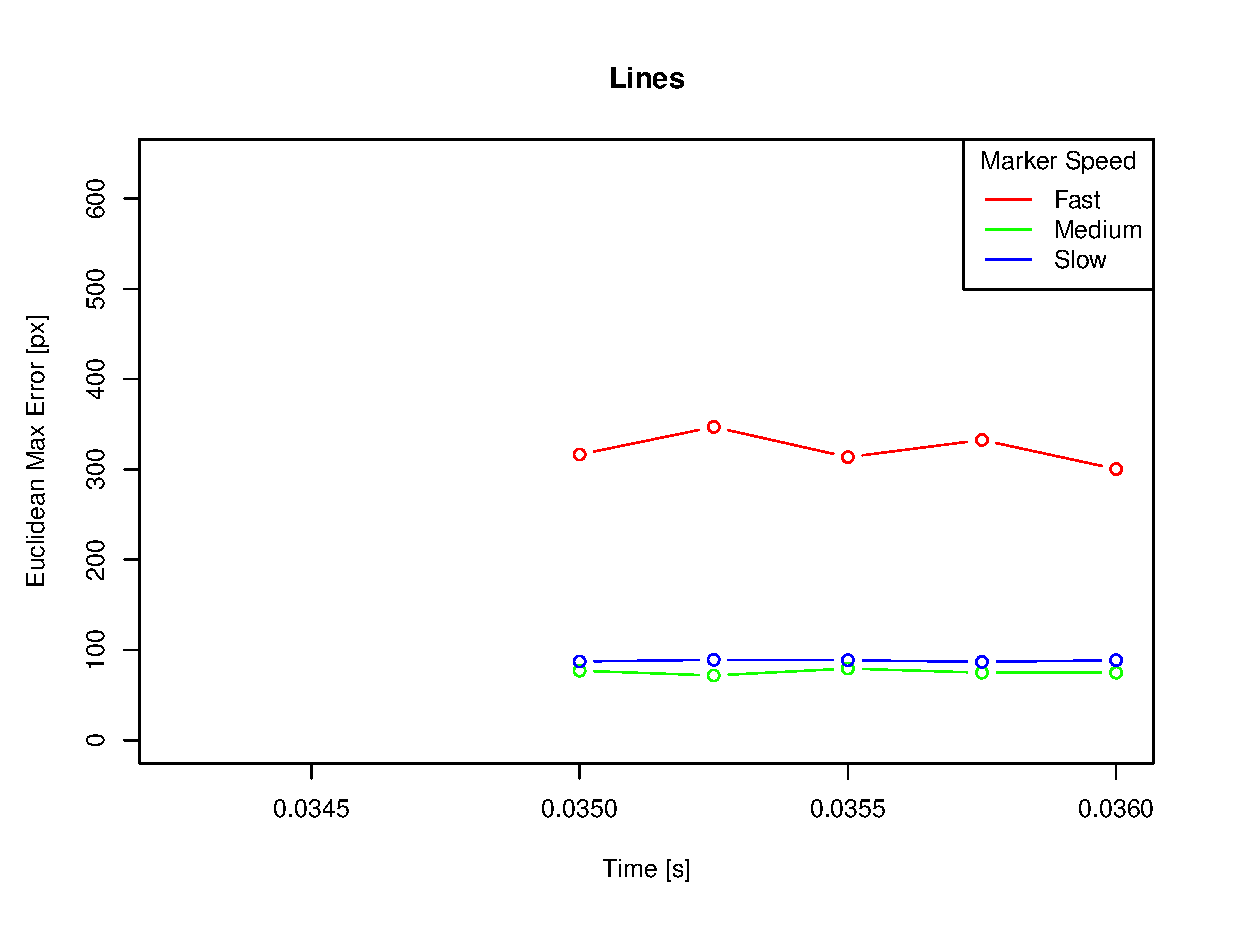
\includegraphics[width= \linewidth]{graphics/robotics/trackingerror_lines}
\caption{Euclidean max error for increasing $\Delta t$ when tracking the line marker.}
\label{fig:trackingerror_lines}
\end{figure}

\begin{figure}[H]
\centering
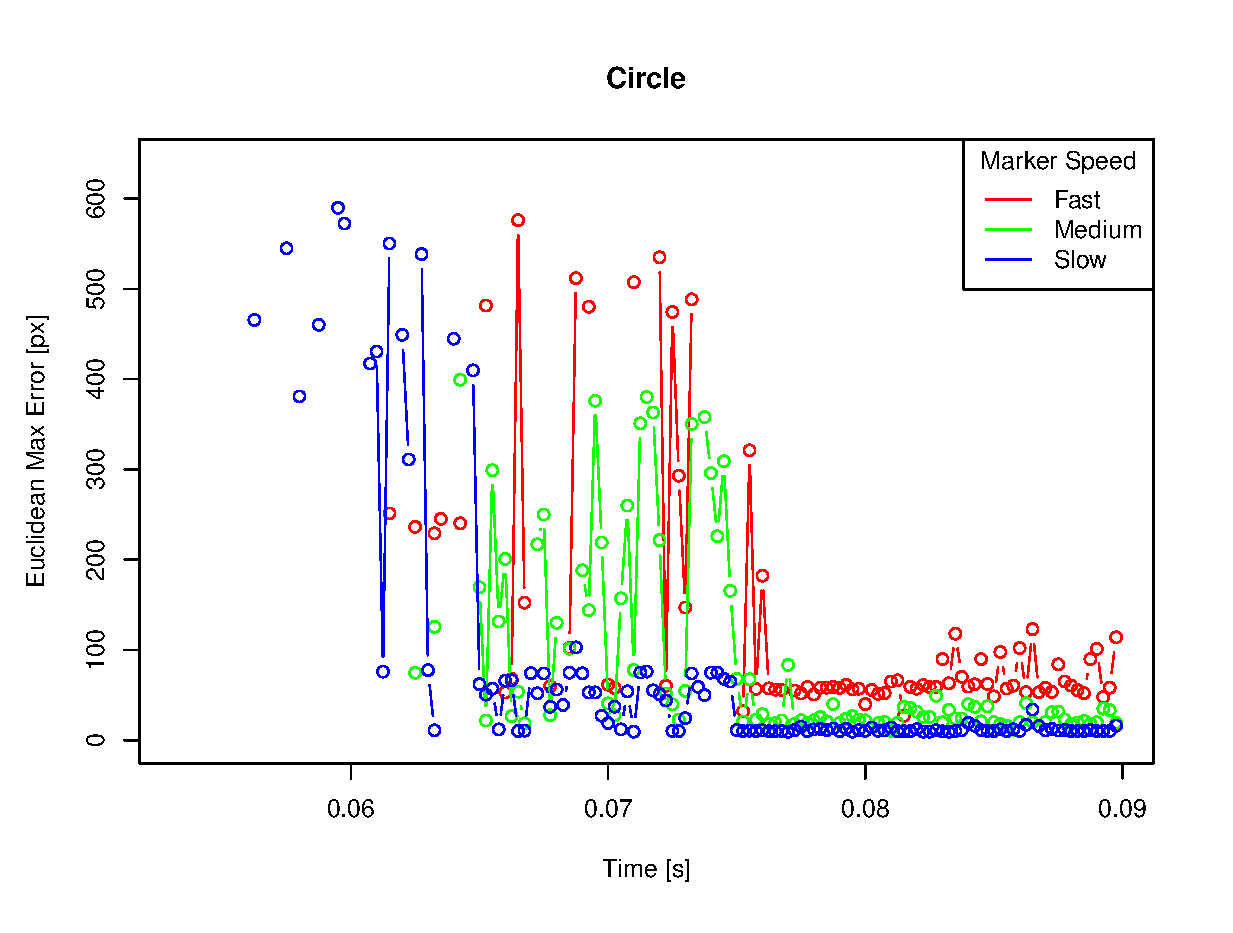
\includegraphics[width= \linewidth]{graphics/robotics/trackingerror_circle}
\caption{Euclidean max error for increasing $\Delta t$ when tracking the circle marker.}
\label{fig:trackingerror_circle}
\end{figure}

\begin{figure}[H]
\centering
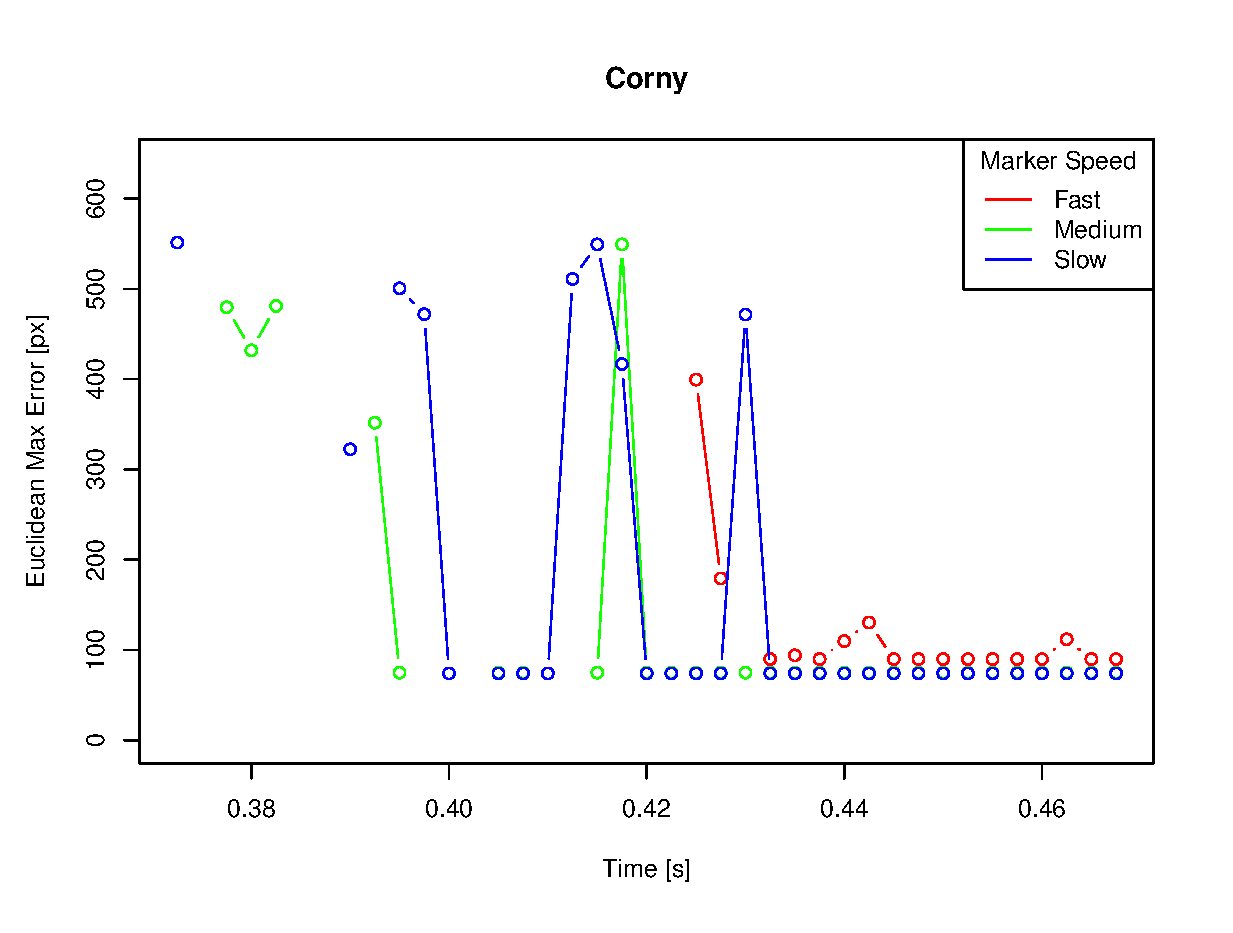
\includegraphics[width= \linewidth]{graphics/robotics/trackingerror_corny}
\caption{Euclidean max error for increasing $\Delta t$ when tracking the corny marker.}
\label{fig:trackingerror_corny}
\end{figure}

Note that the data points were sampled with uniform sample steps, but the data points where the program generated 'not track-able' are not plotted.

As can be seen on figure \ref{fig:trackingerror_circle} 
, then the tracking error has a high fluctuation and lack of data points in the range just before the the sufficient time is reached for which the robot can track the marker.
From the figure the minimum time needed to track the marker reliable can be found.
It is furthermore visible that the point from which the marker can be tracked is approximately the same for all three speeds.
Once this point is reached, the error is approximately constant, but dependent on the marker movement speed.
The breakpoint is around $\Delta t = $ 0.078 [s].
%\ref{fig:trackingerror_lines}, 
%and \ref{fig:trackingerror_corny}

The error when tracking the line was found to be more stable.
As seen in figure \ref{fig:trackingerror_lines}, then there is a sharp change from when it is able to track the marker and when not ($\Delta t = $ 0.035 [s]).
The error for the fast marker speed is first stabilized at a low error after $\Delta t =$ 0.045, whereas the other two are constant throughout.
The final error is generally higher than that of the circle marker, but this is also contributed to by the fact that not the precise center of the marker is found in the vision algorithm.

%The large fluctuation in the maximum error for the Circle algorithm, as seen in figure \ref{fig:trackingerror_circle}, is largely explained by the choice of implementation.
%The default behaviour of the algorithm would only look for circles once in the green channel of the image.
%In worst cases, however, the algorithm finds the hough circles on all three color channels of the image.
%This creates good reasons for the time to variate 



The joint positions can be seen in appendix \ref{app:joint_positions}.
The joint velocities can be seen in appendix \ref{app:joint_velocities}.
\subsection{Conclusion}
The three vision algorithms were successfully implemented into the plug-in and test were performed to describe their performance.
It was found that the robot was able to track the marker for all datasets when the update time is at least 50, 100 and 400 ms for the line, circle and corny images respectively.





\end{document}